\documentclass[a4paper, titlepage]{article}

\usepackage[utf8]{inputenc}
\usepackage[T1]{fontenc}
\usepackage[ngerman]{babel}
\usepackage{graphicx}
\usepackage{hyperref}
\hypersetup{
    colorlinks=true,
    linkcolor=black,
    filecolor=magenta,      
    urlcolor=cyan,
}

\title{React Replacinator}
\author{Damien Flury, Aaron Stampa}
\date{24. Juni 2020}

\begin{document}
  \maketitle
  \begin{abstract}
  Dies ist ein React-Projekt, welches im
  Rahmen des ÜK-Moduls \glqq{}Webtechnologien clientseitig anwenden\grqq{}
  entstanden ist. Das Projekt repräsentiert eine
  minimale React Library, welche es ermöglicht,
  ein Template mit Platzhalter zu verfassen.
  \end{abstract}
  \tableofcontents
  \newpage
  \section{Versionsverwaltung}
  Zur Versionsverwaltung haben wir Github verwendet.
  Darin haben wir mit GitHub Projects gearbeitet,
  um unsere Tasks übersichtlich verwalten zu
  können. Das Repository ist unter 
  \href{https://github.com/DamienFlury/react-replacinator}{React Replacinator}
  verfügbar. In Abbildung \ref{git:commit-history} finden Sie einen Screenshot
  der Commit History.

  \begin{figure}
    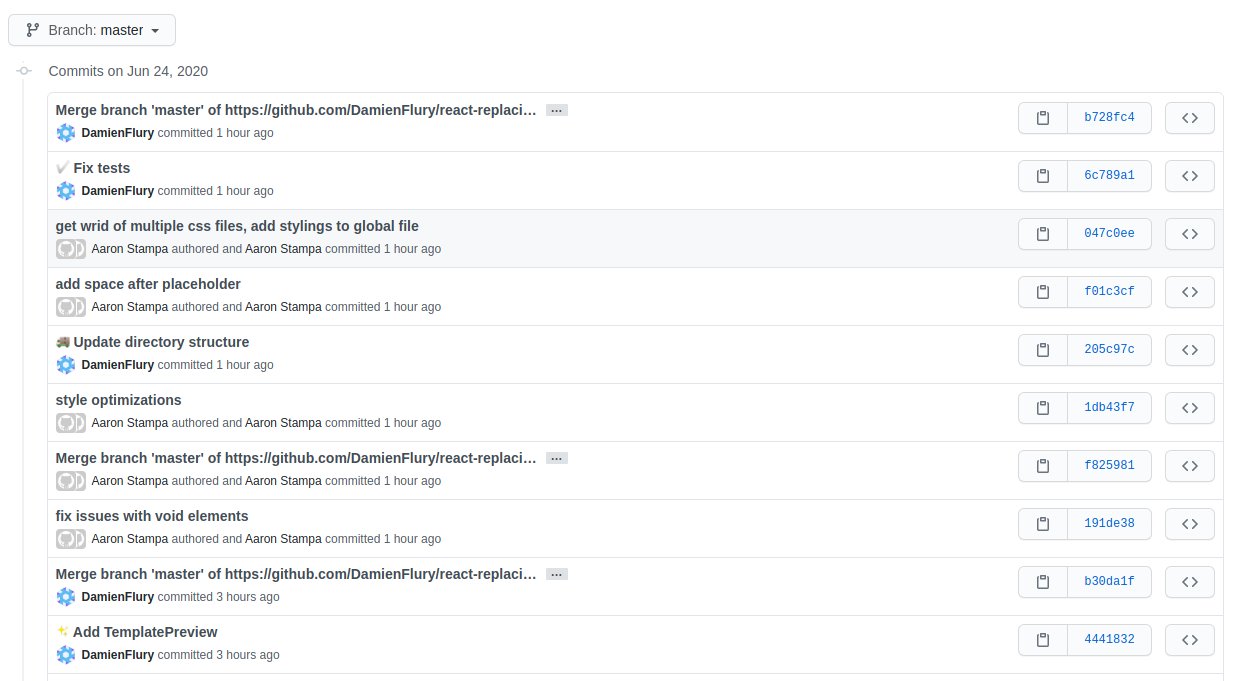
\includegraphics[width=\textwidth]{images/commit-history.png}
    \caption{Commit History}
    \label{git:commit-history}
  \end{figure}
  \section{Idee}
  Die Idee für unser Projekt kam von unserem ÜK-Leiter, der uns mitteilte, 
  lange nach einem Komponenten dieser Art gesucht und noch nichts passendes 
  dazu gefunden habe. 
  Es handelt sich hierbei um eine wiederverwendbare Komponente, mit der man 
  Textvorlagen erstellen kann. Es soll möglich sein, vorgegebene Platzhalter 
  via WYSIWYG in einen Text mit einfachen Klicks einzubinden. 
  Ausserdem soll es eine Preview des fertigen Mails geben.
  \subsection{Komponenten Diagramm}
  Wir verwenden vier Komponenten, wobei eine lediglich
  als Provider dient und somit nur State verwaltet,
  aber die View nicht verändert. Ein Komponentendiagramm
  finden Sie in Abbildung \ref{component-diagram}.
  \begin{figure}
    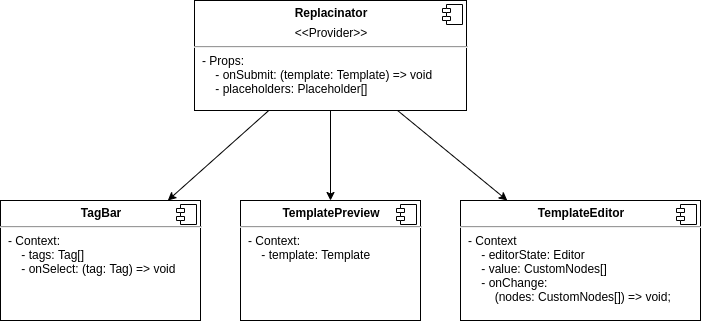
\includegraphics[width=\textwidth]{images/react-replacinator.png}
    \caption{Komponentendiagramm}
    \label{component-diagram}
  \end{figure}
  \section{Anforderungsbeschreibung}
  \subsection{Emailtemplate erstellen}
  \subsection{Preview des Templates darstellen}
  \subsection{Clientschnittstelle zur Verfügung stellen}
  \subsection{}
  \section{Quellcode-Linting}
  Für das Linting des Quellcodes haben wir \emph{ESLint} verwendet.
  Dieses Tool haben wir mit dem Code Formatter \emph{Prettier}
  kombiniert, um Style Guides und Formatting konsistent
  zu halten.
\end{document}